\providecommand{\main}{..}
\documentclass[\main/main.tex]{subfiles}
\begin{document}

\chapter{Come è fatto il tema d'esame}

Un tema d'esame di Ricerca Operativa risulta composto da 4/5 esercizi pratici e talvolta alcune domande di teoria.

\begin{enumerate}
  \item Risolvere graficamento un problema di programmazione lineare a due variabili.
        \subitem Riportare i valori ottenuti (ottimo, variabili, slack).
        \subitem Caratteristiche della soluzione (degenere, multipla).
        \subitem Valore della risorsa $b_i$ per cui la base ottima non cambia.
        \subitem Valore del costo $c_i$ per cui la base ottima non cambia.
        \subitem Risolvere mediante scarti complementari il problema duale.
  \item Data una richiesta, formulare un modello di Programmazione Lineare.
        \subitem Dato il modello realizzato, applicare una data estensione.
  \item Applicare a un grafo l'algoritmo di Ford-Fulkerson.
        \subitem Riportare tutti i cammini aumentati.
        \subitem Calcolare il flusso massimo (quanto flusso arriva alla fine).
        \subitem Determinare il taglio minimo (taglio minimo = insieme di archi che determina strozzatura in massimo flusso).
        \subitem Determinare se il flusso è stato inviato a costo minimo (se esistono circuiti di costo negativo).
        \subitem Si costruisca un reinstradamento che vada a ridurre il costo del flusso.
  \item Applicare Branch \& Bound al problema dello zaino
  \item Problema di programmazione intera:
        \subitem Verificare se una soluzione è ottima per il rilassamento lineare del problema.
        \subitem Risolvere il rilassamento lagrangiano del problema.
        \subitem Taglio di Gomory.
        \subitem Risolvere il duale tramite scarti complementari.
\end{enumerate}

\section{Domande di teoria}

\subsection{Domande su Branch \& Bound}
\begin{figure}
  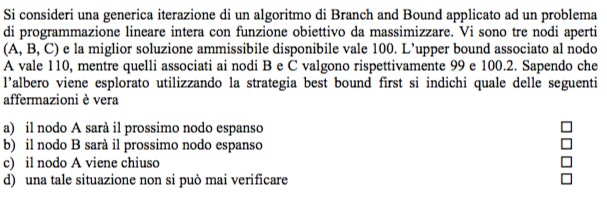
\includegraphics[width=\textwidth]{branch1}
  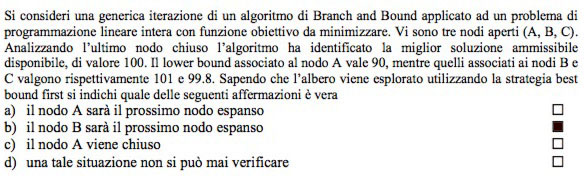
\includegraphics[width=\textwidth]{branch2}
  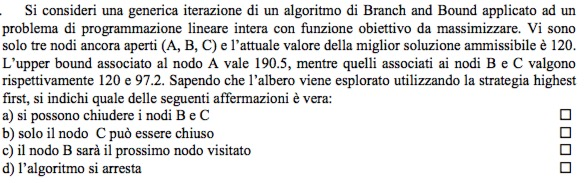
\includegraphics[width=\textwidth]{branch3}
\end{figure}
\subsection{Domande su problema duale}
\begin{figure}
  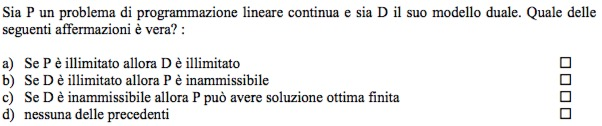
\includegraphics[width=\textwidth]{duale1}
  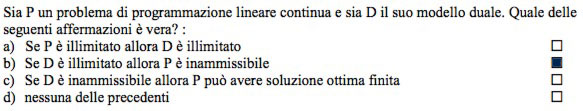
\includegraphics[width=\textwidth]{duale2}
  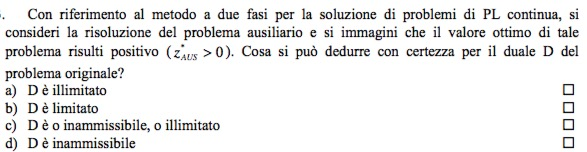
\includegraphics[width=\textwidth]{duale3}
\end{figure}
\subsection{Domande su rilassamento del problema lineare continuo}
\begin{figure}
  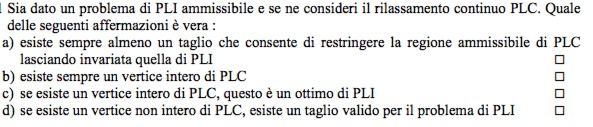
\includegraphics[width=\textwidth]{rilassamentoPLC2}
  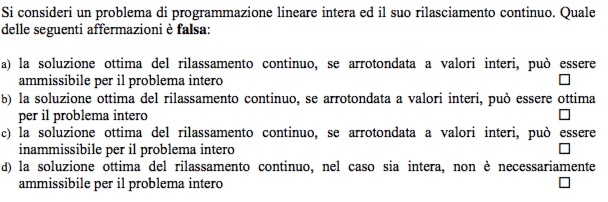
\includegraphics[width=\textwidth]{rilassamentoPLC3}
  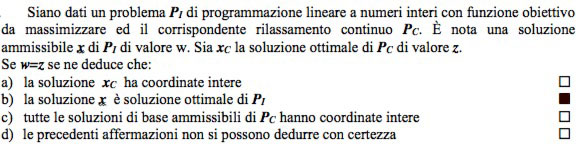
\includegraphics[width=\textwidth]{max3}
\end{figure}
\subsection{Domande su Analisi di sensitività}
\begin{figure}
  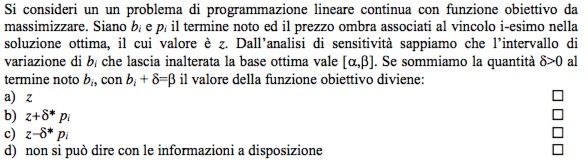
\includegraphics[width=\textwidth]{max2}
  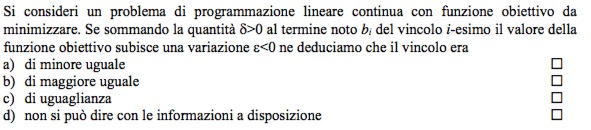
\includegraphics[width=\textwidth]{min1}
\end{figure}
\subsection{Domande varie}
\begin{figure}
  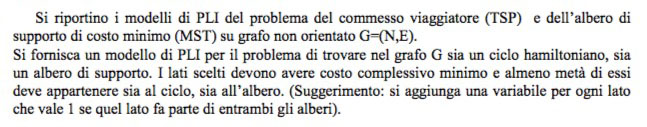
\includegraphics[width=\textwidth]{d6}
\end{figure}
\begin{figure}
  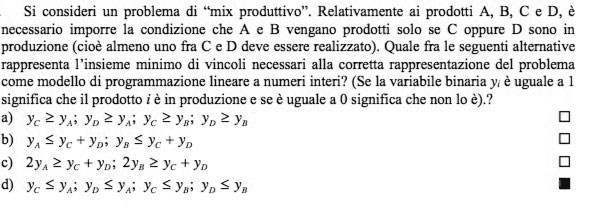
\includegraphics[width=\textwidth]{d7}
\end{figure}

\end{document}